\chapter{Affine and projective plane curves}
\label{ch:affine_projective_riemann}

In this chapter, we will define affine and projective plane curves.
This has two purposes:
\begin{itemize}
	\ii Many interesting curves in $\RR^2$ can be defined as the set of roots of a polynomial.
	This is just a natural generalization.
	\ii We will see that, in fact, \emph{every} compact Riemann surfaces can be written as a
	projective curve! Thus, by studying the projective curves, we have in fact studied all
	compact Riemann surfaces.
\end{itemize}
We will see what these means in the following sections.

\section{Affine plane curves}
Consider some familiar curves on the plane.
\begin{itemize}
	\ii A line can be represented by an equation $y = ax + b$, or $x = c$.
	\ii A circle can be written as the set of $y = \pm \sqrt{1-x^2}$ for $-1 \leq x \leq 1$.
\end{itemize}

There is not much going on so far, but here is a picture.
\begin{center}
	\begin{asy}
		draw((-2, -4)--(2, 4), red, L=Label("$x=2y$", EndPoint, align=E));
		draw(unitcircle, blue, L=Label("$x^2+y^2=1$", Relative(0.13)));
		graph.xaxis("$x$");
		graph.yaxis("$y$");
	\end{asy}
\end{center}

As you can see, the definitions above are actually quite clumsy. We can do better by defining the
points on the curve \emph{implicitly}:
\begin{itemize}
	\ii A line can be represented as the set of $(x, y)$ such that $ax + by + c = 0$.
	\ii A circle can be represented as the set of $(x, y)$ such that $x^2 + y^2 = 1$.
\end{itemize}
Of course, this way it is harder computationally to compute the coordinate of a point,
but the definition is nicer.

The point is:
\begin{moral}
	Many of the interesting curves can be written as the set of roots of a polynomial.
\end{moral}

So we will try to do the same here --- intuitively, if we start with complex dimension $2$ and
specify one polynomial, then the remaining part has complex dimension $1$ i.e. a Riemann surface.

First, there is a technical detail we need to sort out ---
the set of roots of a polynomial need not be a smooth curve.
\begin{example}
	The set of roots of $x^2-y^2 = 0$ in $\RR^2$ is not a curve near the origin --- there are two
	intersecting curves.
	\begin{center}
		\begin{asy}
			draw((-2, -2)--(2, 2), red, L=Label("$x^2-y^2=0$", EndPoint, align=N));
			draw((-2, 2)--(2, -2), red);
			graph.xaxis("$x$");
			graph.yaxis("$y$");
		\end{asy}
	\end{center}
\end{example}

This can be easily handled by placing a restriction on the polynomial.
Let $f(x, y)$ a polynomial, and $X = \{(x, y) \in \RR^2 \mid f(x, y) = 0 \}$. Then:
\begin{theorem}
	For a point $(x, y) \in X$ such that not both
	$\frac{\partial f}{\partial x}$ and $\frac{\partial f}{\partial y}$ vanishes, then $X$
	is smooth near $(x, y)$.
\end{theorem}

If at a point $(x, y) \in X$ such that
$\frac{\partial f}{\partial x} \neq 0$ or $\frac{\partial f}{\partial y} \neq 0$,
we say $X$ is \vocab{smooth} or \vocab{nonsingular} at $(x, y)$.

In fact, we have something more. With notation as above, let $(x, y) \in X$, then:
\begin{itemize}
	\ii Suppose $\frac{\partial f}{\partial x} \neq 0$, then near the point $(x, y)$, $X$ can be
	parametrized by $x = g(y)$ for some analytic function $g$.
	\ii Suppose $\frac{\partial f}{\partial y} \neq 0$, then near the point $(x, y)$, $X$ can be
	parametrized by $y = h(x)$ for some analytic function $h$.
\end{itemize}
All these are just the implicit function theorem.

\begin{exercise}
	Check the statement above on the circle $x^2 + y^2 = 1$, at the points $(0, 1)$ and $(1, 0)$.
\end{exercise}

The exact same statement holds if we replace $\RR^2$ with $\CC^2$.

Next, we want the set of roots $X$ to actually be a \emph{Riemann surface}, not just a set of points
in $\CC^2$. So, we would need to find a suitable analytic structure on $X$.

In the circle above, what would be a suitable analytic structure?
One possible thought is to unroll the circle by arc-length and map it onto $\RR$,
but for a Riemann surface this isn't even well-defined --- how would you unroll, let's say a sphere
onto a plane?

Another possibility is, given the statement of the implicit function above, we declare:
\begin{itemize}
	\ii On an open set $U \subseteq X$ where $\frac{\partial f}{\partial x}\neq 0$ for all points in
	$U$, suppose $U$ is small enough such that $X$ can be parametrized by $x = g(y)$ for some
	analytic function $g$, then the map $\phi$ such that $\phi(x, y) = \phi(g(y), y) = y$ is a
	complex chart.
	\ii Similar for the $\frac{\partial f}{\partial y}\neq 0$ case.
\end{itemize}

A possible complex chart is depicted below. Intuitively, the fact that $\frac{\partial f}{\partial
y}= 0$ at the two points
$(1, 0)$ and $(-1, 0)$
reflects that this ``project-to-$x$'' complex chart cannot be used at these points.
\begin{center}
	\begin{asy}
		size(5cm);
		draw(unitcircle);
		for(real x=-0.95; x<=0.56; x+=0.1){
			real y=sqrt(1-x^2);
			draw((x, y)--(x, 0), blue, Arrow);
			dot((x, y), blue);
			dot((x, 0), blue);
		}
		draw((-0.95, 0)--(0.55, 0), blue);
	\end{asy}
\end{center}

Actually, in the real analytic case, the two definitions above are equivalent.
You can optionally do the exercise below.
\begin{exercise}
	Show this for the circle above. (One possibility is to write down an explicit formula for the
	arc length and show it is analytic)
\end{exercise}

While this definition is already somewhat natural, there is something more to this.
In category theory, we study properties of objects by studying the maps between them.
The set $X$ above has a natural map --- the inclusion map into $\RR^2$, and $\RR^2$ has an obvious
existing analytic structure.

\begin{center}
	\begin{asy}
		size(8cm);
		draw(unitcircle, blue);
		label("$X$", (1, 1)/sqrt(2), blue, align=NE);
		label((1.7, 0), "$\lhook\joinrel\xrightarrow{\quad \iota \quad}$");
		draw(shift(2.4)*scale(3.4)*shift(0, -0.5)*unitsquare);
		label("$\mathbb{R}^2$", shift(2.4)*scale(3.4)*shift(0, -0.5)*(1, 1), align=E);
		draw(shift(2.4)*scale(3.4)*shift(0.5, 0)*scale(1/3.4)*unitcircle, blue);
	\end{asy}
\end{center}

The analytic structure defined above is natural in the following sense:
\begin{itemize}
	\ii For a function $g$ such that $Y \taking g X \taking \iota \RR^2$,
	then $g$ is analytic if and only if $\iota \circ g$ is analytic.
	\ii For a function $X \taking \iota \RR^2 \taking g Y$,
	then $g$ is analytic if and only if $g \circ \iota$ is analytic.
	\ii $X \taking \iota \RR^2$, then $\iota$ is analytic, and
	for any other complex structure $X' \taking{\iota'} \RR^2$ such that $\iota'$ is analytic,
	there exists an unique analytic map $X' \to X$.
\end{itemize}

In fact, each of the bullet point uniquely determines the complex structure on $X$.

In some sense, this is like a universal property for our natural analytic structure.

Of course, we haven't defined what an analytic real manifold is.
Brave readers may try to rigorously formalize all these concepts and prove the statement above.

There is another technical detail that needs to be sorted out. The set of zeros of $f(x, y) =
(y-1)(y-2)$ is:
\begin{center}
	\begin{asy}
		size(4cm);
		import graph;
		draw((-3, 1)--(3, 1), blue);
		draw((-3, 2)--(3, 2), blue);
		graph.xaxis("$x$", -3, 3);
		graph.yaxis("$y$", -3, 3);
	\end{asy}
\end{center}
This is certainly smooth --- but it's not connected. We required a Riemann surface to be connected.

Apart from these two issues, our final statement is:
\begin{definition}
	Given a polynomial $f(z, w) \in \CC[z, w]$, let $X = \{(z, w) \in \CC^2 \mid f(z, w) = 0 \}$
	be the set of roots of $f$.
	Suppose that $X$ is connected, and for all $(z, w) \in X$, $f$ is smooth at $(z, w)$
	(that is, either
	$\frac{\partial f}{\partial z}\neq 0$ or $\frac{\partial f}{\partial w}\neq 0$).
	Then, $X$ is a Riemann surface --- we call $X$ an \vocab{(smooth) affine plane curve},
	with complex charts defined by:
	\begin{itemize}
		\ii On an open set $U$ such that $\frac{\partial f}{\partial z}\neq 0$ everywhere on $U$,
		then $\phi \colon U \to \CC$, $\phi(z, w) = w$ is a complex chart.
		\ii On an open set $U$ such that $\frac{\partial f}{\partial w}\neq 0$ everywhere on $U$,
		then $\phi \colon U \to \CC$, $\phi(z, w) = z$ is a complex chart.
	\end{itemize}
\end{definition}

We call them affine because the plane is ``flat'', unlike the projective plane $\CP^2$ which is
more ``curved'' in some sense.

Of course, we should have some examples --- with these tools, we are in a position to define an
(affine) elliptic curve, and other affine curves.

\begin{example}[A parabola]
	Consider the Riemann surface cut out by $w = z^2$.
	Its real part looks like a parabola:
	\begin{center}
		\begin{asy}
			size(4cm);
			draw(graph.graph(new real(real x){ return x*x; }, -2, 2));
			label((2, 4), "$w=z^2$", align=E);
		\end{asy}
	\end{center}
	Since drawing a graph in $4$ dimensions is difficult, we will project the Riemann surface onto
	$3$ dimensions.
	The result is:
	\begin{center}
		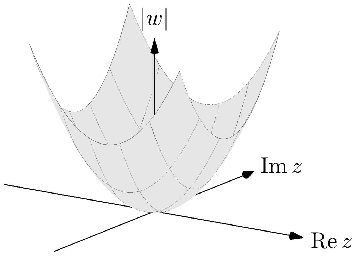
\includegraphics{3dfigures/pdf/parabola.pdf}
	\end{center}

	This Riemann surface is in fact isomorphic to the complex plane $\CC$ by $(z, w) \mapsto z$.
\end{example}

\begin{example}[The circle]
	We all know what the real part of the circle looks like. Visualizing the whole Riemann surface
	is a bit more difficult, however.
	\begin{center}
		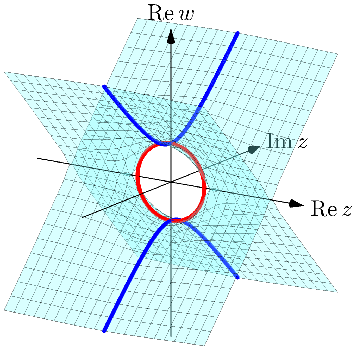
\includegraphics{3dfigures/pdf/circle.pdf}
	\end{center}
	The highlighted red circle is the real part.
	Note that the fact that the plane is shown to be self-intersecting is merely an artifact of the
	projection.

	Although the circle is not isomorphic to the complex plane $\CC$ (we won't be able to prove this
	any time soon\footnote{%
	If you have read the homotopy chapter, this Riemann surface has a deformation retract to its
	real part --- the circle, thus is homotopic to it. We know the complex plane $\CC$ is
	nulhomotopic instead.}),
	it is in fact isomorphic to the hyperbola $x^2-y^2 = 1$
	given by the transformation $y \mapsto y \cdot i$.
	With another rotation and multiplication by a constant,
	it is in turn isomorphic to the hyperbola $xy = 1$,
	which is ``almost'' isomorphic to the line $x = y$, missing one point $(0, 0)$.
\end{example}

\begin{example}[The elliptic curve $y^2 = x^3 - x$]
	The real part looks like this. (The complex part is not drawn this time.)
	\begin{center}
		\begin{asy}
			size(6cm);
			import graph;
			import contour;
			draw(contour(new real(real x, real y){ return x^3-x-y^2; }, (-3,-3), (3, 3),  new real[]{0}), red);
			graph.xaxis("$x$", -3, 3);
			graph.yaxis("$y$", -3, 3);
		\end{asy}
	\end{center}

	While we won't be able to prove this any time soon, turns out this Riemann surface is not
	isomorphic to $\CC$ --- even if we allow deleting finitely many points.
	% (need to check) I only know it's not birationally equivalent because the genus is different
\end{example}

\section{The projective line $\CP^1$}
We will define the projective line --- as it will turn out, it is isomorphic to the Riemann sphere
$\CC_\infty$ which we have already defined. So this section is only to show how our tools work.

As you might have guessed by the name: as a set of points, $\CP^1$ is the quotient of the set of
points $\CC^2 \setminus \{ 0 \}$, modulo the relation $(x, y) \sim (\lambda x, \lambda y)$ for
any $\lambda \in \CC \setminus \{ 0 \}$.

As a topological complex manifold, fortunately, it is still easy --- $\CC^2 \setminus \{ 0 \}$
has a natural topology, and $\CP^1$ gets the quotient topology.
\begin{exercise}
	Define the topology on the space $\RP^1$ analogously.
\end{exercise}
\begin{exercise}
	Let $X \subseteq \RR^2$ be a line that does not pass through the point $(0, 0)$.
	Show that $X \taking f \RR^2 \taking q \RP^1$ is an embedding i.e.
	$X \taking{q \circ f} \img(q \circ f) \subseteq \RP^1$ is a homeomorphism.
\end{exercise}

As a Riemann surface, the usual textbook definition goes:
\begin{definition}[Complex structure of $\CP^1$]
	Cover $\CP^1$ by two open sets, $U_1$ consisting of points with nonzero $x$ coordinate,
	and $U_2$ consisting of points with nonzero $y$-coordinate.
	Then the two complex charts $\phi_1 \colon U_1 \to \CC$ given by $\phi_1(x, y) = y/x$
	and $\phi_2 \colon U_2 \to \CC$ given by $\phi_2(x, y) = x/y$
	determines a complex structure.
\end{definition}
And goes on to prove that the two open sets indeed cover the whole of $\CP^1$,
the value $y/x$ is well-defined, transition maps are holomorphic, etc.

The definition above is elementary, but uninstructive. Where does the complex charts come from?

Given what we have done in the previous chapter, it should be obvious where we should go from here.
There are two things to try:

\begin{itemize}
	\ii Let $X$ be an affine plane curve in $\CC^2$ that does not contain the point $0$.
	Then the map $X \injto \CC^2 \surjto \CP^1$ should be an isomorphism whenever some certain
	derivative does not vanish.
	\ii We can also use maps: the complex structure is such that whenever we have $Y \taking f \CC^2
	\taking q \CP^1$ or $\CC^2 \taking q \CP^1 \taking g Y$, then $f$ is analytic if and only if $q
	\circ f$ is analytic; and $g$ is analytic if and only if $g \circ q$ is analytic.
\end{itemize}

Both are equivalent to the definition above --- in fact, the definition is merely a special case of
the first bullet point, where $X$ is taken to be the line $x = 1$ and $y = 1$ respectively.
Coincidentally, the $2$ resulting complex charts is the simplest one to write down algebraically,
and they already cover the whole $\CP^1$, so it is often taken to be the definition.
There is no reason why it must be these $2$ lines however --- you might as well use $x + y = 1$ and
$x - y = 1$.

\section{Projective plane curves}

Instead of using affine plane curves $X \subseteq \CC^2$, this time around, we will define
projective plane curves $X \subseteq \CP^2$.

Apart from ``just another source of example'', projective plane curves have a distinctive advantage
--- \emph{they're compact}! This allows many nice properties to hold --- we have seen a few in the
last chapter.

We start with defining the \vocab{projective plane} $\CP^2$.
Of course it is $\CC^3 \setminus \{ 0 \}$ quotient by the relation $(x, y, z) \sim (\lambda x,
\lambda y, \lambda z)$.
It has a natural $2$-dimensional complex structure induced from
$\CC^3$ by the quotient map.

The above definition is natural, but abstract. Concretely, we can write:
\begin{ques}
	Define the three complex-manifold charts (on the open set where they're well-defined) by:
	\begin{align*}
		\phi_0(x, y, z) &= (y/x, z/x) \\
		\phi_1(x, y, z) &= (x/y, z/y) \\
		\phi_2(x, y, z) &= (x/z, y/z).
	\end{align*}
	Convince yourself that this complex manifold structure is the correct one.
\end{ques}

Then, a projective plane curve $X$ is defined to be the set of points $(x, y, z)$ such that
$f(x, y, z) = 0$ --- again, satisfying certain smoothness and connectedness conditions.
Unfortunately, if the polynomial were e.g. $f(x, y, z) = x-1$, it will not be well-defined,
as $f(1, 0, 0) = 0$ but $f(2, 0, 0) = 1$.
So we require that $f$ is homogeneous --- that way, $f(x, y, z)$ is still not well-defined, but at
least we know whether $f(x, y, z) = 0$.

The complex structure on a projective plane curve is similarly defined by the universal property.

The definition is short and natural, but abstract. A more concrete definition is given below.
\begin{ques}
	With notation as above, define $U_0$, $U_1$ and $U_2$ to be the domain of $\phi_0$, $\phi_1$ and
	$\phi_2$ respectively.
	Note that $U_i \taking{\phi_i} \CC^2$ gives an isomorphism between $U_i$ and the affine plane
	$\CC^2$.

	Convince yourself that the intersection of a projective plane curve $X$ with one of the $U_i$ is
	a (possibly empty) affine plane curve, when mapped to $\CC^2$, and all the mappings are
	isomorphisms.
\end{ques}

We need some examples.

\begin{example}[The Riemann sphere, again]
	The Riemann sphere can alternatively be defined as the set of points where $z = 0$ in $\CP^2$.

	There's nothing interesting about this --- we already know how the Riemann surface looks like.
	It just serves as a trivial example.
\end{example}

\begin{example}[An elliptic curve, again]
	Let $f(x, y) = x^3-x-y^2$. We know that the set of roots of $f$ in the affine plane $\CC^2$ is
	the elliptic curve.

	Identifying $\CC^2$ with $U_2$, most points in $\CP^2$ can be written as $(x, y, 1)$.
	We want to find a polynomial $g(x, y, z)$ such that its set of roots in $\CP^2$, restricted to
	$U_2$, equals to the elliptic curve.

	Intuitively, by the identity theorem, this should suffices to uniquely determines the Riemann
	surface. Indeed, our target polynomial $g$ is:
	\[ g(x, y, z) = x^3-xz^2-y^2 z.  \]
	This is just the laziest way to homogenize the polynomial $f$, multiplying the least power of
	$z$ to make the result a homogeneous polynomial, and that $g(x, y, 1) = f(x, y)$.

	We have that $\CP^2$ is compact, and the set of roots of $g$ is closed, therefore the resulting
	Riemann surface is \emph{compact}! As promised.
\end{example}

As it turns out, unlike the Riemann sphere, the Riemann surface defined by the elliptic curve above
has \emph{genus 1}!\todo{visualize this} We have the first example that is definitely distinct from
the Riemann sphere.

\begin{exercise}
	In the example above, what if we multiply a larger power of $z$? For instance
	\[ g(x, y, z) = x^3 z-xz^2-y^2 z. \]
\end{exercise}

\begin{example}[A hyperelliptic curve]
	Let $f(x, y) = (x-x_1)(x-x_2) \dotsm (x-x_{2k+1}) - y^2$, where all of $x_1, \dots, x_{2k+1}$ are
	distinct complex numbers.

	We can homogenize $f$ to get $g(x, y, z) = (x-x_1 z)(x-x_2 z) \dotsm (x-x_{2k+1} z) - y^2
	z^{2k-1}$.

	As above, the set of roots of $g$ in $\CP^2$ cuts out a Riemann surface --- once again, this has
	\emph{genus $k$}!

	Therefore, we have seen examples of compact Riemann surfaces of all the genera simply by picking
	different values of $k$.
\end{example}
Saying that we have ``seen'' the surfaces themselves is not quite accurate ---
but you can try to visualize these hyperelliptic curves the same way the elliptic curve is
visualized.

\section{Filling in the holes}
\prototype{The Riemann sphere is formed by filling in a single hole in the complex plane $\CC$.}
\todo{write this}

\section{Nodes of a plane curve}
\prototype{The set defined by the equation $x^2-y^2=0$ has a simple node.}
